\documentclass{article} % For LaTeX2e
\usepackage{nips13submit_e,times}
\usepackage{hyperref}
\usepackage{url}
\usepackage{graphicx}
\graphicspath{ {./} }
%\documentstyle[nips13submit_09,times,art10]{article} % For LaTeX 2.09


\title{SQUAD with BiDAF and DCN}


\author{
Akshay Navalakha \\
\texttt{akshay@stanford.edu} \\
\And
Subin Modeel \\
\texttt{subin@apache.org} \\
}

% The \author macro works with any number of authors. There are two commands
% used to separate the names and addresses of multiple authors: \And and \AND.
%
% Using \And between authors leaves it to \LaTeX{} to determine where to break
% the lines. Using \AND forces a linebreak at that point. So, if \LaTeX{}
% puts 3 of 4 authors names on the first line, and the last on the second
% line, try using \AND instead of \And before the third author name.

\newcommand{\fix}{\marginpar{FIX}}
\newcommand{\new}{\marginpar{NEW}}

\nipsfinalcopy % Uncomment for camera-ready version

\begin{document}


\maketitle

\begin{abstract}
Machine comprehension (MC) and question answering (QA) are related NLP tasks which have seen increased interest with the release of the Stanford Question Answering Dataset (SQuAD). In this paper, we explore 2 neural architecture for the QA task The Bidirectional Attention Flow
model(BiDAF) \& Dynamic Coattention Networks(DCN).We reimplemented the BiDAF and DCN models, compared their attention mechanism. Our best single model achieves an F1 score of  74.524\% F1 and 64.261\% EM on the test set.
\end{abstract}


\section{TODO}
    Title, Author(s)
    Abstract: It should not be more than 300 words.
    
    Introduction: This section introduces the problem, and your overall approach to the problem.
    
    Background/Related Work: This section discusses relevant literature for your project.
    
    Approach: This section details your approach to the problem. For example, this is the section where you would describe the architecture of your neural network. You should be specific - you may want to include equations, figures, plots, etc.
    
    Experiments: In this section, you describe:
        The dataset(s) you used
        How you ran your experiments (e.g. model configurations, learning rate, training time, etc.)
        The evaluation metric(s) you used
        Your results. It's very important to show both quantitative evaluation (show numbers, figures, tables etc. relating to your evaluation metric(s)) and qualitative evaluation (show example results, etc.). 
        
    Conclusion: What have you learned? Suggest future ideas.
    
    References: Include references to all literature that informed your project work. This is absolutely necessary.


\section{Introduction}

Question answering (QA) is a task in natural language processing that requires both natural language understanding and world knowledge. In this task, a model must give answers to queries presented in natural language based on a context paragraph.The context contains the answer to the query.
Most of the QA datasets were high in quality due to human annotation, but small in size (Berant et al., 2014; Richardson et al., 2013). Hence, they did not allow for training data-intensive, expressive models such as deep neural networks.

To address this problem, researchers have developed large-scale datasets through semi-automated techniques (Hermann et al., 2015; Hill et al., 2016). Compared to their smaller, hand-annotated counterparts, these QA datasets allow the training of more expressive models. However, it has been shown that they differ from more natural, human annotated datasets in the types of reasoning required to answer the questions (Chen et al., 2016).

Recently, Rajpurkar et al. (2016) released the Stanford Question Answering dataset (SQuAD), which is orders of magnitude larger than all previous hand-annotated datasets and has a variety of qualities that culminate in a natural QA task. SQuAD has the desirable quality that answers are spans in a reference document. This constrains answers to the space of all possible spans. However, Rajpurkar et al. (2016) show that the dataset retains a diverse set of answers and requires different forms of logical reasoning, including multi-sentence reasoning.

We explored 2 neural architecture for the QA task The Bidirectional Attention Flow model(BiDAF) \& Dynamic Coattention Networks(DCN).

Dynamic Coattention model [3], exploits the deep learning technique of attention.Here we compute the affinity matrix between the context and question, which is then used to weight the continuous representations of the two documents.The decoder layer is complicated where it iteratively  estimates the start and end location of the answer, allowing it to better handle local minima. 

Bi-Directional Attention Flow (BiDAF)[2] model  has a encoder similar to the Dynamic Coattention model[3] where they first compute an affinity matrix which is used to compute both context-to-query and query-to-context attention. However, the decoder and output layers for BiDAF are much simpler.
We focussed on these last two papers in creating our models for the QA task.

\section{Background}

We use pre-trained GloVe vectors to represent the words in the context and question.Let \( x^{Q}_{1} , x^{Q}_{2} , . . . , x^{Q}_{n} \)  denote words in the question and \(x^{D}_{1} , x^{D}_{2} , . . . , x^{D}_{m} \) denote the same for words in the context.

\subsection{BiDAF}

BiDAF  model is a hierarchical multi-stage process and consists of six layers:
\begin{enumerate}
\item Character Embedding Layer maps each word to a vector space using character-level CNNs.
\item Word Embedding Layer maps each word to a vector space using a pre-trained word em- bedding model.
\item Contextual Embedding Layer utilizes contextual cues from surrounding words to refine the embedding of the words. These first three layers are applied to both the query and context.
\item Attention Flow Layer couples the query and context vectors and produces a set of query- aware feature vectors for each word in the context.
\item Modeling Layer employs a Recurrent Neural Network to scan the context. 6. Output Layer provides an answer to the query.
\end{enumerate}


Assume we have context hidden states $c_1, . . . , c_N \ \epsilon \  R^{2h} $ and question hidden states $q_1, . . . , q_M \ \epsilon \  R^{2h} $. We compute the similarity matrix S ∈ RN ×M , which contains a similarity score Sij for each pair (ci,qj) of context and question hidden states.
S =wT [c;q;c◦q]∈R ij sim i j i j
Here, ci ◦ qj is an elementwise product and wsim ∈ R6h is a weight vector.
Next, we perform Context-to-Question (C2Q) Attention. (This is similar to our baseline’s Attention Layer). We take the row-wise softmax of S to obtain attention distributions αi, which we use to take weighted sums of the question hidden states qj, yielding C2Q attention outputs ai.
In equations, this is:
αi = softmax(Si,:) ∈ RM ∀i ∈ {1,...,N} M
ai =  αjiqj ∈ R2h ∀i ∈ {1,...,N} j=1
Next, we perform Question-to-Context(Q2C) Attention. For each context location i ∈ {1, . . . , N }, we take the max of the corresponding row of the similarity matrix, mi = maxj Sij ∈ R. Then we take the softmax over the resulting vector m ∈ RN – this gives us an attention distribution β ∈ RN over context locations. We then use β to take a weighted sum of the context hidden states ci – this is the Q2C attention output c′. In equations:
mi = maxSij ∈ R ∀i ∈ {1,...,N} j
β = softmax(m) ∈ RN N
c′ = βici ∈R2h i=1
(1)
Lastly, for each context location i ∈ {1,...,N} we obtain the output bi of the Bidirectional Attention Flow Layer by combining the context hidden state ci, the C2Q attention output ai, and
10
the Q2C attention output c′:
$$bi =[ci;ai;ci ◦ai;ci ◦c′]∈R8h ∀i∈{1,...,N}$$
where ◦ represents elementwise multiplication.


\begin{math}\epsilon\end{math}
\subsection{DCN}

\subsubsection{Encoder}
We encode the Context as : $d_{t} = LSTM_{enc} \langle d_{t-1},x^{D}_{t} \rangle $ using a LSTM. 
We define the context encoding matrix as $ D = \langle d_{1} ...d_{m},d_{\emptyset} \rangle $ $ \ \epsilon \  R^{l\times(m+1)} $.
We also add a sentinel vector $ d_{\emptyset} $ (Merity et al., 2016), which we later show allows the model to not attend to any particular word in the input.

The question embeddings are computed with the same LSTM to share representation power: $ q_{t} =LSTM_{enc} \langle q_{t-1} , x^{Q}_{t} \rangle $ .
We define an intermediate question representation $ Q′ = \langle q_{1} . . . q_{n},q_{\emptyset} \rangle $ $ \ \epsilon \  R^{l\times(n+1)} $.
To allow for variation between the question encoding space and the document encod- ing space, we introduce a non-linear projection layer on top of the question encoding. 
The final representation for the question becomes: $ Q = tanh \langle   W^Q Q′ + b^Q \rangle \  \epsilon \  R^{l\times(n+1)} $


\subsubsection{Coattention Decoder}
The coattention mechanism  attends to the question and document simultaneously, similar to (Lu et al., 2016), and finally fuses both attention contexts. Figure 2 provides an illustration of the coattention encoder.
We first compute the affinity matrix, which contains affinity scores corresponding to all pairs of document words and question words: $ L = D^{T}Q \ \epsilon \  R^{(m+1)\times(n+1)} $. The affinity matrix is nor-
malized row-wise to produce the attention weights $A^{Q}$ across the document for each word in the question, and column-wise to produce the attention weights $A^{D}$ across the question for each word in the document:
$$A^{Q} = softmax (L) \  \epsilon \ R^{(m+1)\times(n+1)} \ and \  A^{D} = softmax(L^{T}) \ \epsilon \ R^{(n+1)\times(m+1)}  $$
Next, we compute the summaries, or attention contexts, of the document in light of each word of the question.
$$C^{Q} = DA^{Q} \  \epsilon \  R^{l\times(n+1)}$$


We similarly compute the summaries $QA^{D}$ of the question in light of each word of the document. Similar to Cui et al. (2016), we also compute the summaries $C^{Q}A^{D}$ of the previous attention con- texts in light of each word of the document. These two operations can be done in parallel, as is shown in Eq. 3. One possible interpretation for the operation $C^{Q}A^{D}$ is the mapping of question encoding into space of document encodings.
$$C^{D} = [Q;C^{Q}] A^{D} \ \epsilon \ R^{2l\times(m+1)}$$. We define $C^{D}$, a co-dependent representation of the question and document, as the coattention
context. We use the notation $[a; b]$ for concatenating the vectors a and b horizontally.
The last step is the fusion of temporal information to the coattention context via a bidirectional
LSTM: $$
u_{t} = BiLSTM ( u_{t−1}, u_{t+1},  [d_{t}; c^{D}_{t}])    \ \epsilon \  R^{2l}.$$ We define $U =[u_1,...,u_m]\ \epsilon \ R^{2l \times m} $ ,which provides a foundation for selecting which span may
be the best possible answer, as the coattention encoding.


\section{Experiments}
\begin{figure}
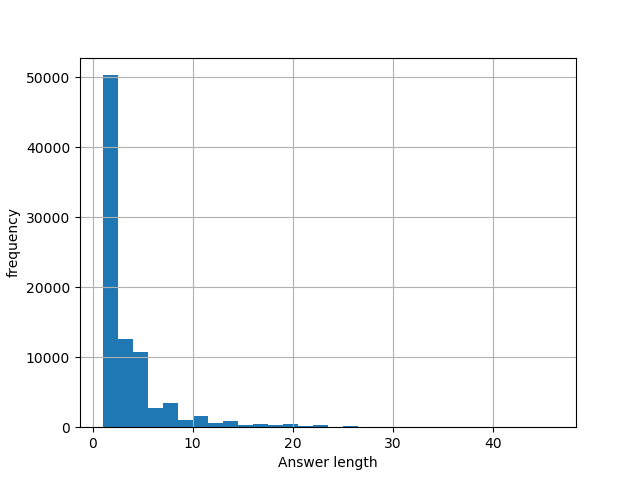
\includegraphics[scale=.65]{template/Answer.png}
\centering
\end{figure}



\begin{figure}
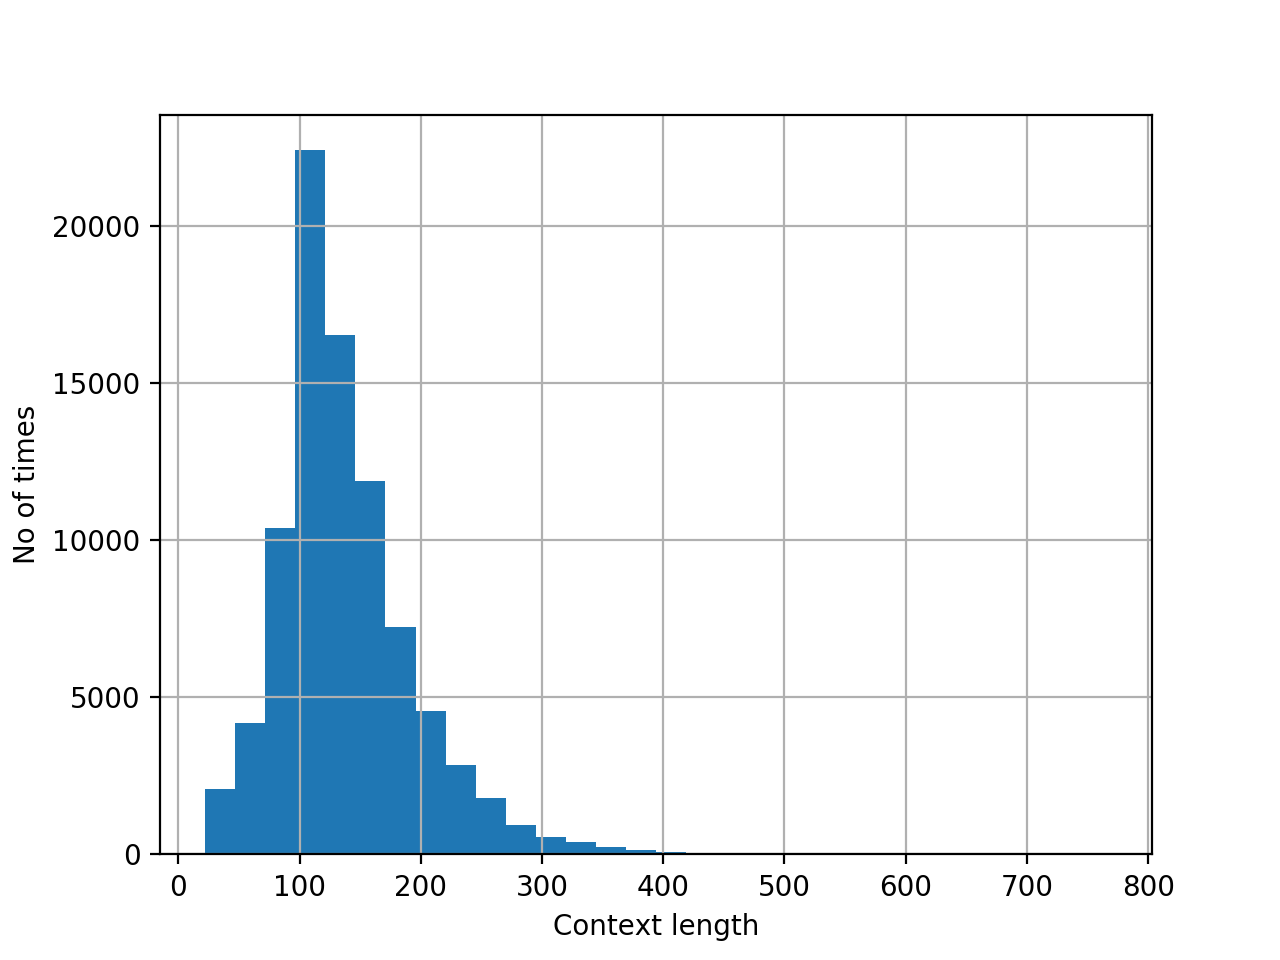
\includegraphics[scale=.65]{template/Context.png}
\centering
\end{figure}

 

\section{Conclusion}

We were able to build a good model for answering questions presented to it in natural language. Of the 4 models we developed our BiDAF model was able to achieve better performance.
As of right now, we achieve a F1 score of 74.1 and an EM score of 64.1, which is on par with some of the entries on the official SQuAD leaderboard.


\subsection*{Future Work}

There are a few more experiments we would like to try in the future.We would like to replace the BiDAF Decoder with DCN Pointer decoder, which is able to recover from local maxima.Also, Try other modifications like using more word features.
The original BiDAF implementation used character encoding which was not implemented by us and there is still scope for further hyperparameter
tuning and bug fixing.

\section{Acknowledgments}

We would like to thank Richard Socher, and all the TAs for this course.
We would also like to give our thanks to Microsoft for providing GPUs on Azure to train our models.

\section*{References}

\small{

[1] P. Rajpurkar, J. Zhang, K. Lopyrev, and P. Liang, “Squad: 100,000+ questions for machine comprehension of text,” arXiv preprint \href{https://arxiv.org/abs/1606.05250}{arXiv:1606.05250}, 2016.

[2] M. Seo, A. Kembhavi, A. Farhadi, and H. Hajishirzi, “Bidirectional attention flow for machine comprehension,” arXiv preprint \href{https://arxiv.org/abs/1611.01603}{arXiv:1611.01603}, 2016.

[3] C. Xiong, V. Zhong, and R. Socher, “Dynamic coattention networks for question answering,” arXiv preprint \href{https://arxiv.org/abs/1611.01604}{arXiv:1611.01604}, 2016.

[4] J. Pennington, R. Socher, and C. D. Manning, “Glove: Global vectors for word representation.,” in EMNLP, vol. 14,\href{https://nlp.stanford.edu/pubs/glove.pdf}{pp. 1532–1543}, 2014.

}

\end{document}
